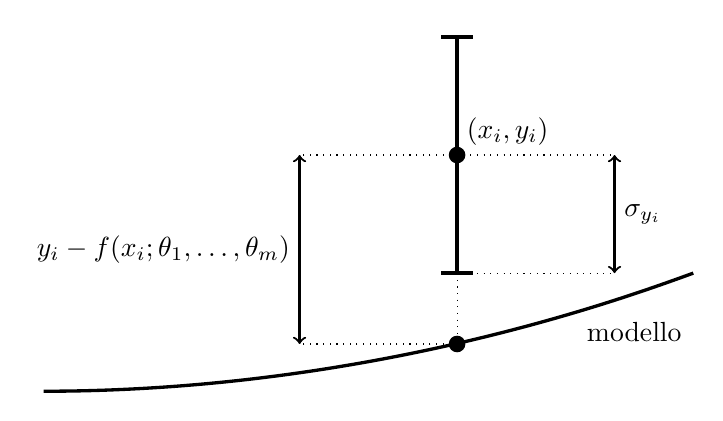
\begin{tikzpicture}
  \node at (0, 0) {};
  \pgfmathsetmacro{\x}{3.}
  \pgfmathsetmacro{\dx}{0.2}
  \pgfmathsetmacro{\qx}{2.0}
  \pgfmathsetmacro{\dy}{1.5}
  \draw[very thick] (\x, 0) -- (\x, -2*\dy);
  \draw[very thick] (\x-\dx, 0) -- (\x+\dx, 0);
  \draw[very thick] (\x-\dx, -2*\dy) -- (\x+\dx, -2*\dy);
  \fill (\x, -\dy) circle [radius=3pt];
  \node[anchor=south west] at (\x, -\dy) {$(x_i, y_i)$};
  \draw[style=dotted] (\x, -\dy) -- (\x + \qx, -\dy);
  \draw[style=dotted] (\x, -2*\dy) -- (\x + \qx, -2*\dy);
  \draw[thick,{<[scale=1.5]}-{>[scale=1.5]}]
  (\x + \qx, -\dy) -- (\x + \qx, -2*\dy);
  \node[anchor=west] at (\x + \qx, -1.5*\dy) {$\sigma_{y_i}$};
  \draw[very thick] (-0.75*\x, -3*\dy) parabola (2*\x,-2*\dy);
  \fill (\x, -2.6*\dy) circle [radius=3pt];
  \draw[style=dotted] (\x, -2*\dy) -- (\x, -2.6*\dy);
  \draw[style=dotted] (\x, -\dy) -- (\x - \qx, -\dy);
  \draw[style=dotted] (\x, -2.6*\dy) -- (\x - \qx, -2.6*\dy);
  \draw[thick,{<[scale=1.5]}-{>[scale=1.5]}]
  (\x - \qx, -\dy) -- (\x - \qx, -2.6*\dy);
  \node[anchor=east] at (\x - \qx, -1.8*\dy)
       {$y_i - f(x_i; \theta_1,\ldots,\theta_m)$};
  \node at (1.75*\x, -2.5*\dy) {modello};
\end{tikzpicture}
